\chapter{BLAST}
\label{chapter:blast}
Hey, everybody loves BLAST right? I mean, geez, how can it get any easier to do comparisons between one of your sequences and every other sequence in the known world? But, of course, this section isn't about how cool BLAST is, since we already know that. It is about the problem with BLAST -- it can be really difficult to deal with the volume of data generated by large runs, and to automate BLAST runs in general.

Fortunately, the Biopython folks know this only too well, so they've developed lots of tools for dealing with BLAST and making things much easier. This section details how to use these tools and do useful things with them.

Dealing with BLAST can be split up into two steps, both of which can be done from within Biopython.
Firstly, running BLAST for your query sequence(s), and getting some output.
Secondly, parsing the BLAST output in Python for further analysis.

Your first introduction to running BLAST was probably via the NCBI web-service.
In fact, there are lots of ways you can run BLAST, which can be categorized in several ways.
The most important distinction is running BLAST locally (on your own machine),
and running BLAST remotely (on another machine, typically the NCBI servers).
We're going to start this chapter by invoking the NCBI online BLAST service
from within a Python script.

\emph{NOTE}: The following Chapter~\ref{chapter:searchio} describes
\verb|Bio.SearchIO|, an \emph{experimental} module in Biopython. We
intend this to ultimately replace the older \verb|Bio.Blast| module, as it
provides a more general framework handling other related sequence
searching tools as well. However, until that is declared stable, for
production code please continue to use the  \verb|Bio.Blast| module
for dealing with NCBI BLAST.

\section{Running BLAST over the Internet}
\label{sec:running-www-blast}

We use the function \verb|qblast()| in the \verb|Bio.Blast.NCBIWWW| module
to call the online version of BLAST.  This has three non-optional arguments:
\begin{itemize}
\item The first argument is the blast program to use for the search, as a
lower case string. The options and descriptions of the programs are
available at \url{https://blast.ncbi.nlm.nih.gov/Blast.cgi}.
Currently \verb|qblast| only works with blastn, blastp, blastx, tblast
and tblastx.
\item The second argument specifies the databases to search against. Again,
the options for this are available on the NCBI Guide to BLAST
\url{ftp://ftp.ncbi.nlm.nih.gov/pub/factsheets/HowTo_BLASTGuide.pdf}.
\item The third argument is a string containing your query sequence.  This
can either be the sequence itself, the sequence in fasta format,
or an identifier like a GI number.
\end{itemize}

The \verb|qblast| function also take a number of other option arguments
which are basically analogous to the different parameters you can set
on the BLAST web page.  We'll just highlight a few of them here:

\begin{itemize}
\item The argument \verb|url_base| sets the base URL for running BLAST over the
internet. By default it connects to the NCBI, but one can use this to connect
to an instance of NCBI BLAST running in the cloud. Please refer to the documentation
for the \verb|qblast| function for further details.
\item The \verb|qblast| function can return the BLAST results in various
formats, which you can choose with the optional \verb|format_type| keyword:
\verb|"HTML"|, \verb|"Text"|, \verb|"ASN.1"|, or \verb|"XML"|.
The default is \verb|"XML"|, as that is the format expected by the parser,
described in section~\ref{sec:parsing-blast} below.
\item The argument \verb|expect| sets the expectation or e-value threshold.
\end{itemize}

For more about the optional BLAST arguments, we refer you to the NCBI's own
documentation, or that built into Biopython:

\begin{minted}{pycon}
>>> from Bio.Blast import NCBIWWW
>>> help(NCBIWWW.qblast)
\end{minted}

Note that the default settings on the NCBI BLAST website are not quite
the same as the defaults on QBLAST. If you get different results, you'll
need to check the parameters (e.g., the expectation value threshold and
the gap values).

For example, if you have a nucleotide sequence you want to search against
the nucleotide database (nt) using BLASTN, and you know the GI number of your
query sequence, you can use:

\begin{minted}{pycon}
>>> from Bio.Blast import NCBIWWW
>>> result_handle = NCBIWWW.qblast("blastn", "nt", "8332116")
\end{minted}

Alternatively, if we have our query sequence already in a FASTA formatted
file, we just need to open the file and read in this record as a string,
and use that as the query argument:

\begin{minted}{pycon}
>>> from Bio.Blast import NCBIWWW
>>> fasta_string = open("m_cold.fasta").read()
>>> result_handle = NCBIWWW.qblast("blastn", "nt", fasta_string)
\end{minted}

We could also have read in the FASTA file as a \verb|SeqRecord| and then
supplied just the sequence itself:

\begin{minted}{pycon}
>>> from Bio.Blast import NCBIWWW
>>> from Bio import SeqIO
>>> record = SeqIO.read("m_cold.fasta", format="fasta")
>>> result_handle = NCBIWWW.qblast("blastn", "nt", record.seq)
\end{minted}

Supplying just the sequence means that BLAST will assign an identifier
for your sequence automatically.  You might prefer to use the
\verb|SeqRecord| object's format method to make a FASTA string
(which will include the existing identifier):

\begin{minted}{pycon}
>>> from Bio.Blast import NCBIWWW
>>> from Bio import SeqIO
>>> record = SeqIO.read("m_cold.fasta", format="fasta")
>>> result_handle = NCBIWWW.qblast("blastn", "nt", record.format("fasta"))
\end{minted}

This approach makes more sense if you have your sequence(s) in a
non-FASTA file format which you can extract using \verb|Bio.SeqIO|
(see Chapter~\ref{chapter:seqio}).

Whatever arguments you give the \verb|qblast()| function, you should
get back your results in a handle object (by default in XML format).
The next step would be to parse the XML output into Python objects
representing the search results (Section~\ref{sec:parsing-blast}),
but you might want to save a local copy of the output file first.
I find this especially useful when debugging my code that extracts
info from the BLAST results (because re-running the online search
is slow and wastes the NCBI computer time).

\label{sec:saving-blast-output}

We need to be a bit careful since we can use \verb|result_handle.read()| to
read the BLAST output only once -- calling \verb|result_handle.read()| again
returns an empty string.

\begin{minted}{pycon}
>>> with open("my_blast.xml", "w") as out_handle:
...     out_handle.write(result_handle.read())
...
>>> result_handle.close()
\end{minted}

After doing this, the results are in the file \verb|my_blast.xml| and the
original handle has had all its data extracted (so we closed it). However,
the \verb|parse| function of the BLAST parser (described
in~\ref{sec:parsing-blast}) takes a file-handle-like object, so
we can just open the saved file for input:

\begin{minted}{pycon}
>>> result_handle = open("my_blast.xml")
\end{minted}

Now that we've got the BLAST results back into a handle again, we are ready
to do something with them, so this leads us right into the parsing section
(see Section~\ref{sec:parsing-blast} below). You may want to jump ahead to
that now \ldots.

\section{Running BLAST locally}
\label{sec:running-local-blast}

\subsection{Introduction}

Running BLAST locally (as opposed to over the internet, see
Section~\ref{sec:running-www-blast}) has at least major two advantages:
\begin{itemize}
\item Local BLAST may be faster than BLAST over the internet;
\item Local BLAST allows you to make your own database to search for sequences against.
\end{itemize}
Dealing with proprietary or unpublished sequence data can be another reason to run BLAST
locally.  You may not be allowed to redistribute the sequences, so submitting them to the
NCBI as a BLAST query would not be an option.

Unfortunately, there are some major drawbacks too -- installing all the bits and getting
it setup right takes some effort:
\begin{itemize}
\item Local BLAST requires command line tools to be installed.
\item Local BLAST requires (large) BLAST databases to be setup (and potentially kept up to date).
\end{itemize}

\noindent
To further confuse matters there are several different BLAST packages available,
and there are also other tools which can produce imitation BLAST output files, such as BLAT.

\subsection{Standalone NCBI BLAST+}

The ``new''
\href{https://blast.ncbi.nlm.nih.gov/Blast.cgi?CMD=Web&PAGE_TYPE=BlastDocs&DOC_TYPE=Download}
{NCBI BLAST+} suite was released in 2009. This replaces the old NCBI ``legacy'' BLAST
package (see below).

This section will show briefly how to use these tools from within Python. If you have
already read or tried the alignment tool examples in Section~\ref{sec:alignment-tools}
this should all seem quite straightforward. First, we construct a command line string
(as you would type in at the command line prompt if running standalone BLAST by hand).
Then we can execute this command from within Python.

For example, taking a FASTA file of gene nucleotide sequences, you might want to
run a BLASTX (translation) search against the non-redundant (NR) protein database.
Assuming you (or your systems administrator) has downloaded and installed the NR
database, you might run:

\begin{minted}{console}
$ blastx -query opuntia.fasta -db nr -out opuntia.xml -evalue 0.001 -outfmt 5
\end{minted}

This should run BLASTX against the NR database, using an expectation cut-off value
of $0.001$ and produce XML output to the specified file (which we can then parse).
On my computer this takes about six minutes - a good reason to save the output
to a file so you can repeat any analysis as needed.

From within python we can use the \verb|subprocess| module to build the command line
string, and run it:

\begin{minted}{pycon}
>>> import subprocess
>>> cmd = "blastx -query opuntia.fasta -db nr -out opuntia.xml"
>>> cmd += " -evalue 0.001 -outfmt 5"
>>> subprocess.run(cmd, shell=True)
\end{minted}

In this example there shouldn't be any output from BLASTX to the terminal. You may want
to check the output file \verb|opuntia.xml| has been created.

As you may recall from earlier examples in the tutorial, the \verb|opuntia.fasta|
contains seven sequences, so the BLAST XML output should contain multiple results.
Therefore use \verb|Bio.Blast.NCBIXML.parse()| to parse it as described below in
Section~\ref{sec:parsing-blast}.

\subsection{Other versions of BLAST}

NCBI BLAST+ (written in C++) was first released in 2009 as a replacement for
the original NCBI ``legacy'' BLAST (written in C) which is no longer being updated.
There were a lot of changes -- the old version had a single core command line
tool \verb|blastall| which covered multiple different BLAST search types (which
are now separate commands in BLAST+), and all the command line options
were renamed.
Biopython's wrappers for the NCBI ``legacy'' BLAST tools have been deprecated
and will be removed in a future release.
To try to avoid confusion, we do not cover calling these old tools from Biopython
in this tutorial.

You may also come across \href{http://blast.wustl.edu/}{Washington University BLAST}
(WU-BLAST), and its successor, \href{https://blast.advbiocomp.com}{Advanced Biocomputing
BLAST} (AB-BLAST, released in 2009, not free/open source). These packages include
the command line tools \verb|wu-blastall| and \verb|ab-blastall|, which mimicked
\verb|blastall| from the NCBI ``legacy'' BLAST suite.
Biopython does not currently provide wrappers for calling these tools, but should be able
to parse any NCBI compatible output from them.

\section{Parsing BLAST output}
\label{sec:parsing-blast}

As mentioned above, BLAST can generate output in various formats, such as
XML, HTML, and plain text. Originally, Biopython had parsers for BLAST
plain text and HTML output, as these were the only output formats offered
at the time. Unfortunately, the BLAST output in these formats kept changing,
each time breaking the Biopython parsers. Our HTML BLAST parser has been
removed, while the deprecated plain text BLAST parser is now only available
via \verb|Bio.SearchIO|. Use it at your own risk, it may or may not work,
depending on which BLAST version you're using.

As keeping up with changes in BLAST
became a hopeless endeavor, especially with users running different BLAST
versions, we now recommend to parse the output in XML format, which can be
generated by recent versions of BLAST. Not only is the XML output more stable
than the plain text and HTML output, it is also much easier to parse
automatically, making Biopython a whole lot more stable.

You can get BLAST output in XML format in various ways. For the parser, it
doesn't matter how the output was generated, as long as it is in the XML format.
\begin{itemize}
\item You can use Biopython to run BLAST over the internet, as described in
section~\ref{sec:running-www-blast}.
\item You can use Biopython to run BLAST locally, as described in
section~\ref{sec:running-local-blast}.
\item You can do the BLAST search yourself on the NCBI site through your
web browser, and then save the results. You need to choose XML as the format
in which to receive the results, and save the final BLAST page you get
(you know, the one with all of the interesting results!) to a file.
\item You can also run BLAST locally without using Biopython, and save
the output in a file. Again, you need to choose XML as the format in which
to receive the results.
\end{itemize}
The important point is that you do not have to use Biopython
scripts to fetch the data in order to be able to parse it.
Doing things in one of these ways, you then need to get a handle
to the results. In Python, a handle is just a nice general way of
describing input to any info source so that the info can be retrieved
using \verb|read()| and \verb|readline()| functions
(see Section~\ref{sec:appendix-handles}).

If you followed the code above for interacting with BLAST through a
script, then you already have \verb|result_handle|, the handle to the
BLAST results.  For example, using a GI number to do an online search:

\begin{minted}{pycon}
>>> from Bio.Blast import NCBIWWW
>>> result_handle = NCBIWWW.qblast("blastn", "nt", "8332116")
\end{minted}

If instead you ran BLAST some other way, and have the
BLAST output (in XML format) in the file \verb|my_blast.xml|, all you
need to do is to open the file for reading:

\begin{minted}{pycon}
>>> result_handle = open("my_blast.xml")
\end{minted}

Now that we've got a handle, we are ready to parse the output. The
code to parse it is really quite small.  If you expect a single
BLAST result (i.e., you used a single query):

\begin{minted}{pycon}
>>> from Bio.Blast import NCBIXML
>>> blast_record = NCBIXML.read(result_handle)
\end{minted}

\noindent or, if you have lots of results (i.e., multiple query sequences):

\begin{minted}{pycon}
>>> from Bio.Blast import NCBIXML
>>> blast_records = NCBIXML.parse(result_handle)
\end{minted}

Just like \verb|Bio.SeqIO| and \verb|Bio.AlignIO|
(see Chapters~\ref{chapter:seqio} and~\ref{chapter:align}),
we have a pair of input functions, \verb|read| and \verb|parse|, where
\verb|read| is for when you have exactly one object, and \verb|parse|
is an iterator for when you can have lots of objects -- but instead of
getting \verb|SeqRecord| or \verb|MultipleSeqAlignment| objects, we
get BLAST record objects.

To be able to handle the situation where the BLAST file may be huge,
containing thousands of results, \verb|NCBIXML.parse()| returns an
iterator. In plain English, an iterator allows you to step through
the BLAST output, retrieving BLAST records one by one for each BLAST
search result:

\begin{minted}{pycon}
>>> from Bio.Blast import NCBIXML
>>> blast_records = NCBIXML.parse(result_handle)
>>> blast_record = next(blast_records)
# ... do something with blast_record
>>> blast_record = next(blast_records)
# ... do something with blast_record
>>> blast_record = next(blast_records)
# ... do something with blast_record
>>> blast_record = next(blast_records)
Traceback (most recent call last):
  File "<stdin>", line 1, in <module>
StopIteration
# No further records
\end{minted}

Or, you can use a \verb|for|-loop:
\begin{minted}{pycon}
>>> for blast_record in blast_records:
...     pass  # Do something with blast_record
...
\end{minted}

Note though that you can step through the BLAST records only once.
Usually, from each BLAST record you would save the information that
you are interested in. If you want to save all returned BLAST records,
you can convert the iterator into a list:
\begin{minted}{pycon}
>>> blast_records = list(blast_records)
\end{minted}
Now you can access each BLAST record in the list with an index as usual.
If your BLAST file is huge though, you may run into memory problems trying to
save them all in a list.

Usually, you'll be running one BLAST search at a time. Then, all you need
to do is to pick up the first (and only) BLAST record in \verb|blast_records|:
\begin{minted}{pycon}
>>> from Bio.Blast import NCBIXML
>>> blast_records = NCBIXML.parse(result_handle)
>>> blast_record = next(blast_records)
\end{minted}
\noindent or more elegantly:
\begin{minted}{pycon}
>>> from Bio.Blast import NCBIXML
>>> blast_record = NCBIXML.read(result_handle)
\end{minted}

I guess by now you're wondering what is in a BLAST record.

\section{The BLAST record class}

A BLAST Record contains everything you might ever want to extract from the
BLAST output. Right now we'll just show
an example of how to get some info out of the BLAST report, but if you
want something in particular that is not described here, look at the
info on the record class in detail, and take a gander into the code or
automatically generated documentation -- the docstrings have lots of
good info about what is stored in each piece of information.

To continue with our example, let's just print out some summary info
about all hits in our blast report greater than a particular
threshold. The following code does this:

\begin{minted}{pycon}
>>> E_VALUE_THRESH = 0.04

>>> for alignment in blast_record.alignments:
...     for hsp in alignment.hsps:
...         if hsp.expect < E_VALUE_THRESH:
...             print("****Alignment****")
...             print("sequence:", alignment.title)
...             print("length:", alignment.length)
...             print("e value:", hsp.expect)
...             print(hsp.query[0:75] + "...")
...             print(hsp.match[0:75] + "...")
...             print(hsp.sbjct[0:75] + "...")
...
\end{minted}

This will print out summary reports like the following:

\begin{minted}{text}
****Alignment****
sequence: >gb|AF283004.1|AF283004 Arabidopsis thaliana cold acclimation protein WCOR413-like protein
alpha form mRNA, complete cds
length: 783
e value: 0.034
tacttgttgatattggatcgaacaaactggagaaccaacatgctcacgtcacttttagtcccttacatattcctc...
||||||||| | ||||||||||| || ||||  || || |||||||| |||||| |  | |||||||| ||| ||...
tacttgttggtgttggatcgaaccaattggaagacgaatatgctcacatcacttctcattccttacatcttcttc...
\end{minted}

Basically, you can do anything you want to with the info in the BLAST
report once you have parsed it. This will, of course, depend on what
you want to use it for, but hopefully this helps you get started on
doing what you need to do!

An important consideration for extracting information from a BLAST report is the type of objects that the information is stored in. In Biopython, the parsers return \verb|Record| objects, either \verb|Blast| or \verb|PSIBlast| depending on what you are parsing. These objects are defined in \verb|Bio.Blast.Record| and are quite complete.

Here are my attempts at UML class diagrams for the \verb|Blast| and \verb|PSIBlast| record classes. If you are good at UML and see mistakes/improvements that can be made, please let me know. The Blast class diagram is shown in Figure~\ref{fig:blastrecord}.

\begin{htmlonly}
\label{fig:blastrecord}
\imgsrc[width=650, height=750]{images/BlastRecord.png}
\end{htmlonly}

\begin{latexonly}
\begin{figure}[htbp]
\centering
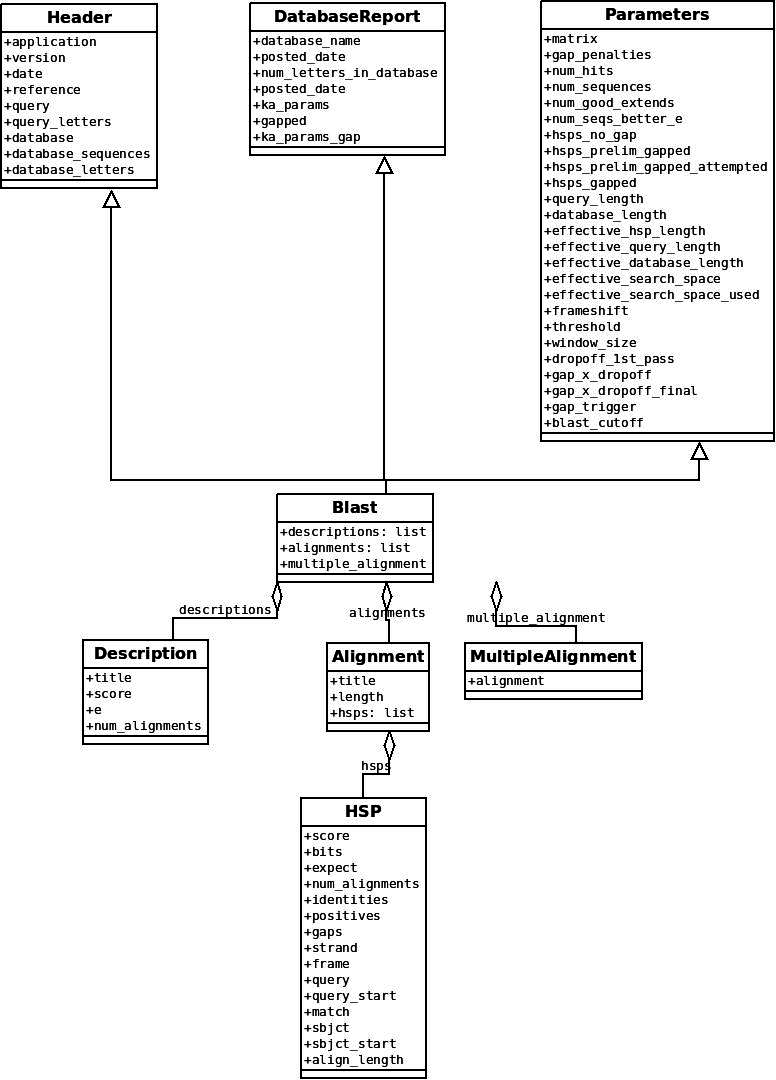
\includegraphics[width=0.8\textwidth]{images/BlastRecord.png}
\caption{Class diagram for the Blast Record class representing all of the info in a BLAST report}
\label{fig:blastrecord}
\end{figure}
\end{latexonly}

The PSIBlast record object is similar, but has support for the rounds that are used in the iteration steps of PSIBlast. The class diagram for PSIBlast is shown in Figure~\ref{fig:psiblastrecord}.

\begin{htmlonly}
\label{fig:psiblastrecord}
\imgsrc[width=650, height=750]{images/PSIBlastRecord.png}
\end{htmlonly}

\begin{latexonly}
\begin{figure}[htbp]
\centering
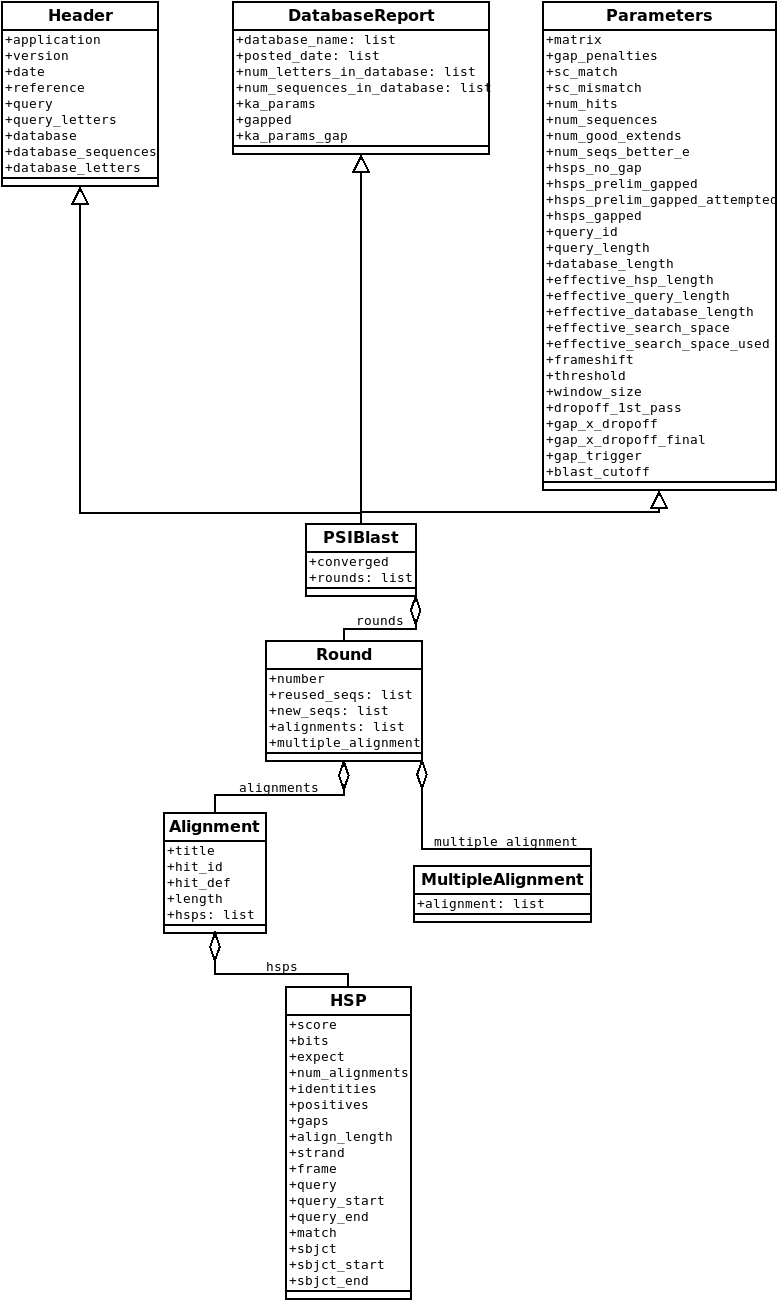
\includegraphics[width=0.8\textwidth]{images/PSIBlastRecord.png}
\caption{Class diagram for the PSIBlast Record class.}
\label{fig:psiblastrecord}
\end{figure}
\end{latexonly}


\section{Dealing with PSI-BLAST}

You can run the standalone version of PSI-BLAST (the legacy NCBI command line
tool \verb|blastpgp|, or its replacement \verb|psiblast|) directly from the
command line or using python's \verb|subprocess| module.

At the time of writing, the NCBI do not appear to support tools running a
PSI-BLAST search via the internet.

Note that the \verb|Bio.Blast.NCBIXML| parser can read the XML output from
current versions of PSI-BLAST, but information like which sequences in each
iteration is new or reused isn't present in the XML file.

\section{Dealing with RPS-BLAST}

You can run the standalone version of RPS-BLAST (either the legacy NCBI
command line tool \verb|rpsblast|, or its replacement with the same name)
directly from the command line or using python's \verb|subprocess| module.

At the time of writing, the NCBI do not appear to support tools running an
RPS-BLAST search via the internet.

You can use the \verb|Bio.Blast.NCBIXML| parser to read the XML output from
current versions of RPS-BLAST.
